% !TEX TS-program = pdflatex
% !TEX encoding = UTF-8 Unicode

% This is a simple template for a LaTeX document using the "article" class.
% See "book", "report", "letter" for other types of document.

\documentclass[11pt]{article} % use larger type; default would be 10pt

\usepackage[utf8]{inputenc} % set input encoding (not needed with XeLaTeX)

%%% Examples of Article customizations
% These packages are optional, depending whether you want the features they provide.
% See the LaTeX Companion or other references for full information.

%%% PAGE DIMENSIONS
\usepackage{geometry} % to change the page dimensions
\geometry{a4paper} % or letterpaper (US) or a5paper or....
% \geometry{margin=2in} % for example, change the margins to 2 inches all round
% \geometry{landscape} % set up the page for landscape
%   read geometry.pdf for detailed page layout information

\usepackage{graphicx} % support the \includegraphics command and options

% \usepackage[parfill]{parskip} % Activate to begin paragraphs with an empty line rather than an indent

%%% PACKAGES
\usepackage{booktabs} % for much better looking tables
\usepackage{array} % for better arrays (eg matrices) in maths
\usepackage{paralist} % very flexible & customisable lists (eg. enumerate/itemize, etc.)
\usepackage{verbatim} % adds environment for commenting out blocks of text & for better verbatim
\usepackage{subfig} % make it possible to include more than one captioned figure/table in a single float
% These packages are all incorporated in the memoir class to one degree or another...

%%% HEADERS & FOOTERS
\usepackage{fancyhdr} % This should be set AFTER setting up the page geometry
\pagestyle{fancy} % options: empty , plain , fancy
\renewcommand{\headrulewidth}{0pt} % customise the layout...
\lhead{}\chead{}\rhead{}
\lfoot{}\cfoot{\thepage}\rfoot{}

%%% SECTION TITLE APPEARANCE
\usepackage{sectsty}
\allsectionsfont{\sffamily\mdseries\upshape} % (See the fntguide.pdf for font help)
% (This matches ConTeXt defaults)

%%% ToC (table of contents) APPEARANCE
\usepackage[nottoc,notlof,notlot]{tocbibind} % Put the bibliography in the ToC
\usepackage[titles,subfigure]{tocloft} % Alter the style of the Table of Contents
\renewcommand{\cftsecfont}{\rmfamily\mdseries\upshape}
\renewcommand{\cftsecpagefont}{\rmfamily\mdseries\upshape} % No bold!

\usepackage{graphicx}
\graphicspath{ {image/} }

%%% END Article customizations

%%% The "real" document content comes below...

\title{CS 698: Assignment 2}
\author{Ronghao Yang}
%\date{} % Activate to display a given date or no date (if empty),
         % otherwise the current date is printed 

\begin{document}
\maketitle

\section{Question 1}
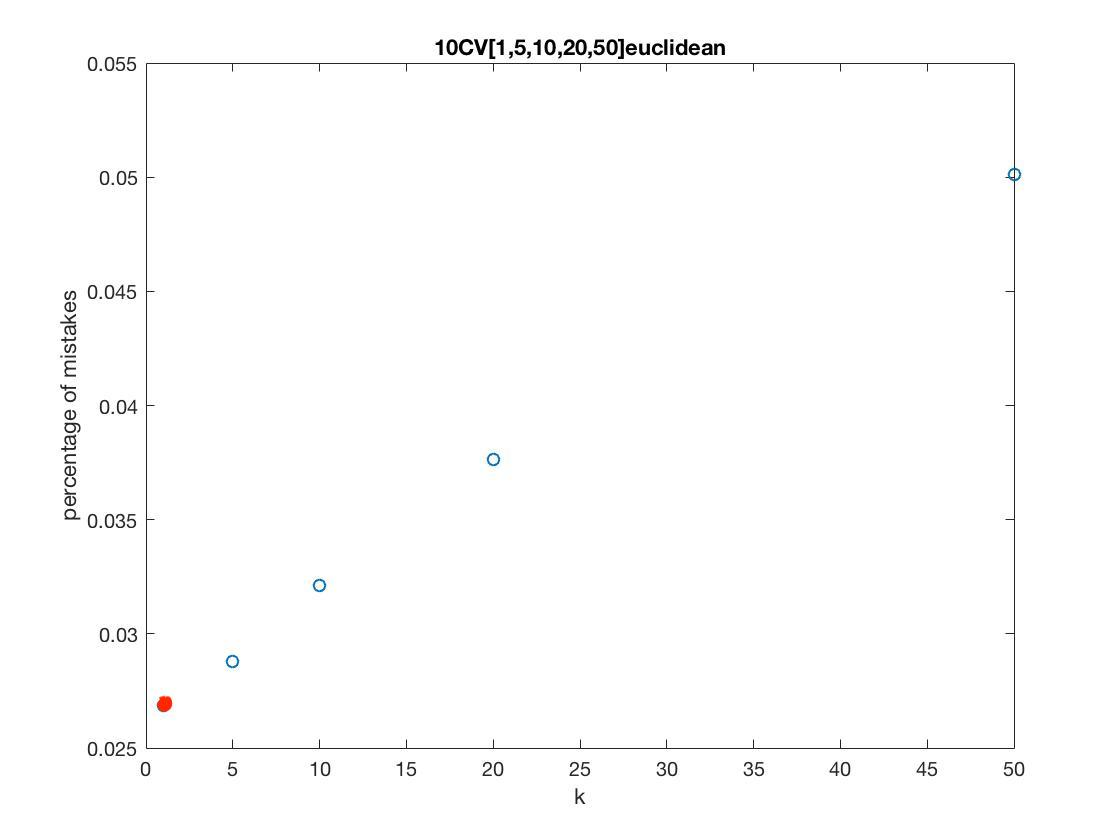
\includegraphics[scale=0.4]{10CV[1,5,10,20,50]euclidean.jpg}\\\linebreak
For the first case, we set k to be 1, 5, 10, 20, 50, and the distance metric to be $euclidean distance$. When using 10-fold cross validation on the training set, the optimal k is 1. When using k=1 on the testing set, the error rate is 3.09\%\\
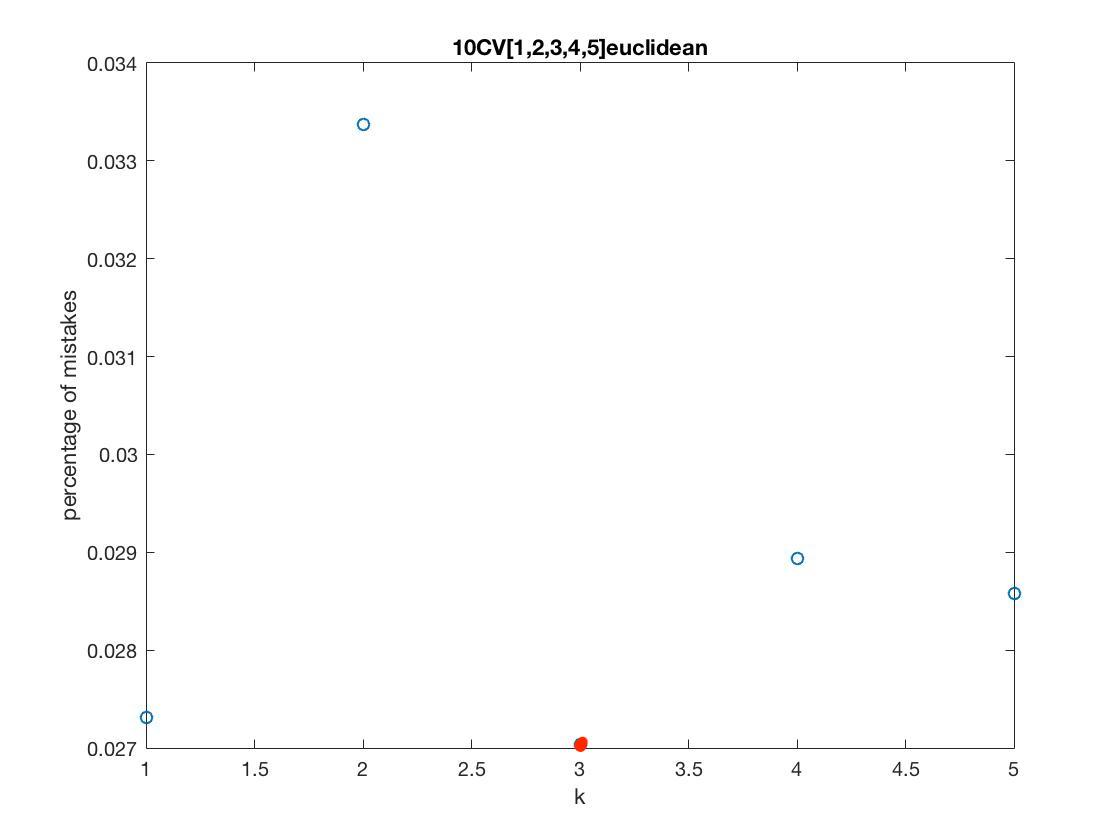
\includegraphics[scale=0.4]{10CV[1,2,3,4,5]euclidean.jpg}\\
For the second case, we set k to be 1, 2, 3, 4, 5, and the distance metric to be $euclidean distance$. When using 10-fold cross validation on the training set, the optimal k is 3. When using k=3 on the testing set, the error rate is 2.95\%\\
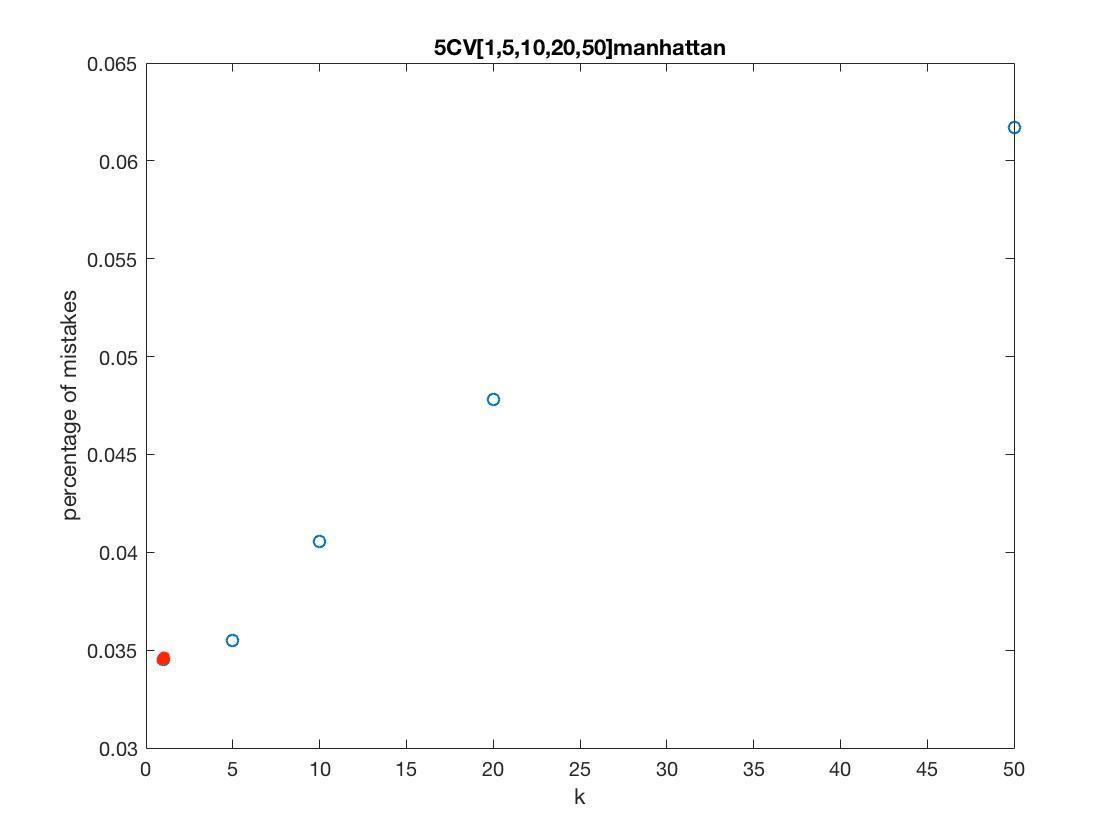
\includegraphics[scale=0.4]{5CV[1,5,10,20,50]manhattan.jpg}\\
For the first case, we set k to be 1, 5, 10, 20, 50, and the distance metric to be $manhattan distance$. When using 5-fold cross validation on the training set, the optimal k is 1. When using k=1 on the testing set, the error rate is 3.69\%\\
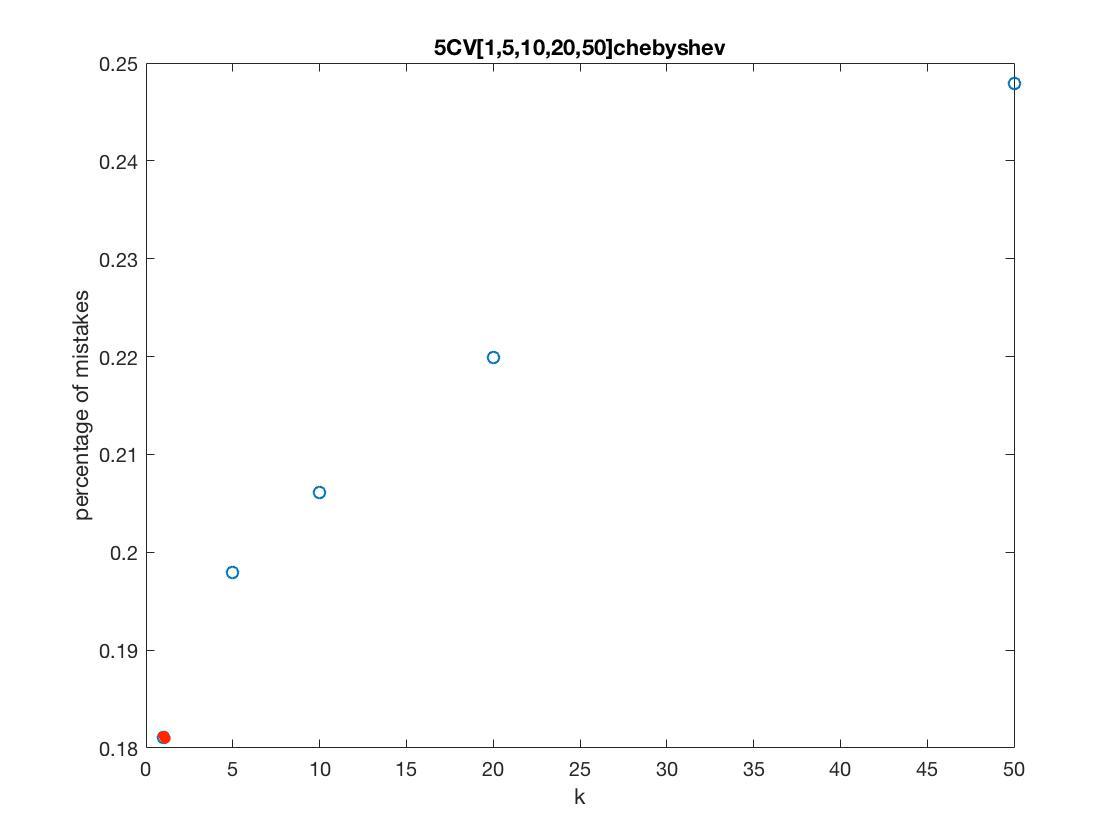
\includegraphics[scale=0.4]{5CV[1,5,10,20,50]chebyshev.jpg}\\
For the first case, we set k to be 1, 5, 10, 20, 50, and the distance metric to be $chebyshev distance$. When using 10-fold cross validation on the training set, the optimal k is 1. When using k=1 on the testing set, the error rate is 17.41\%\\\linebreak\linebreak

\section{Question 2}
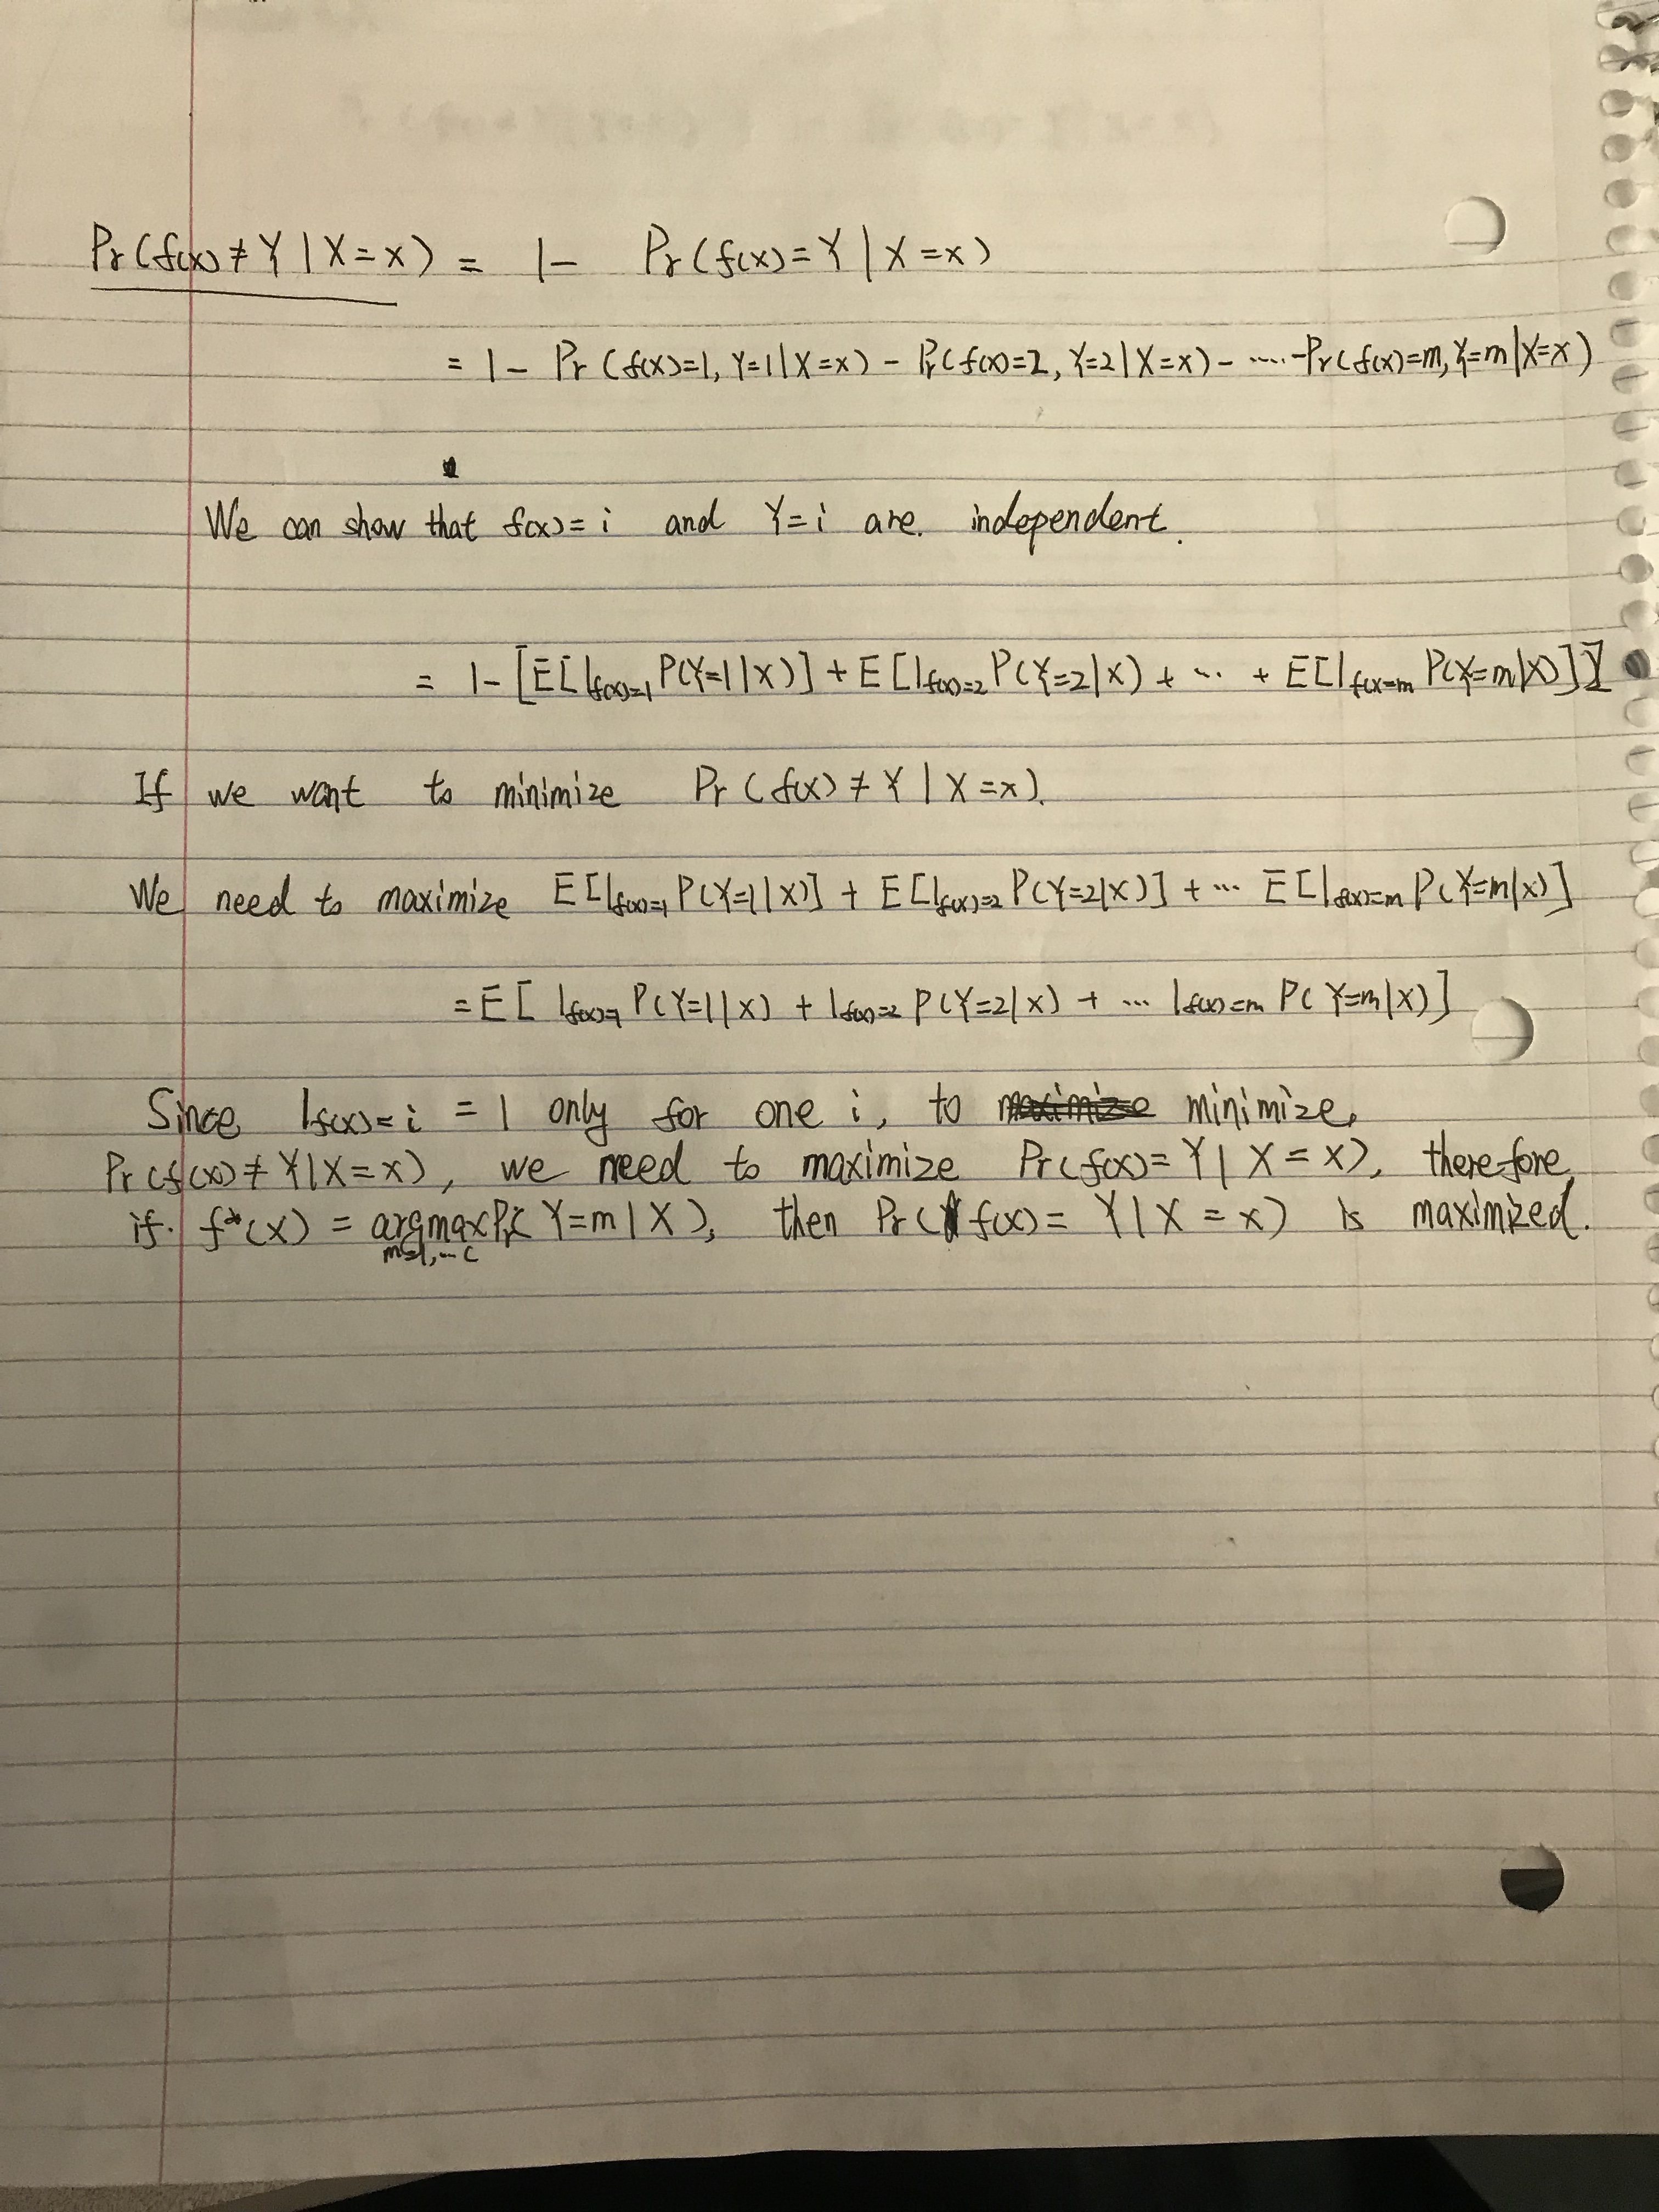
\includegraphics[scale=0.15]{q2.jpeg}]


\section{Question 3}
\subsection{Question 3.1}
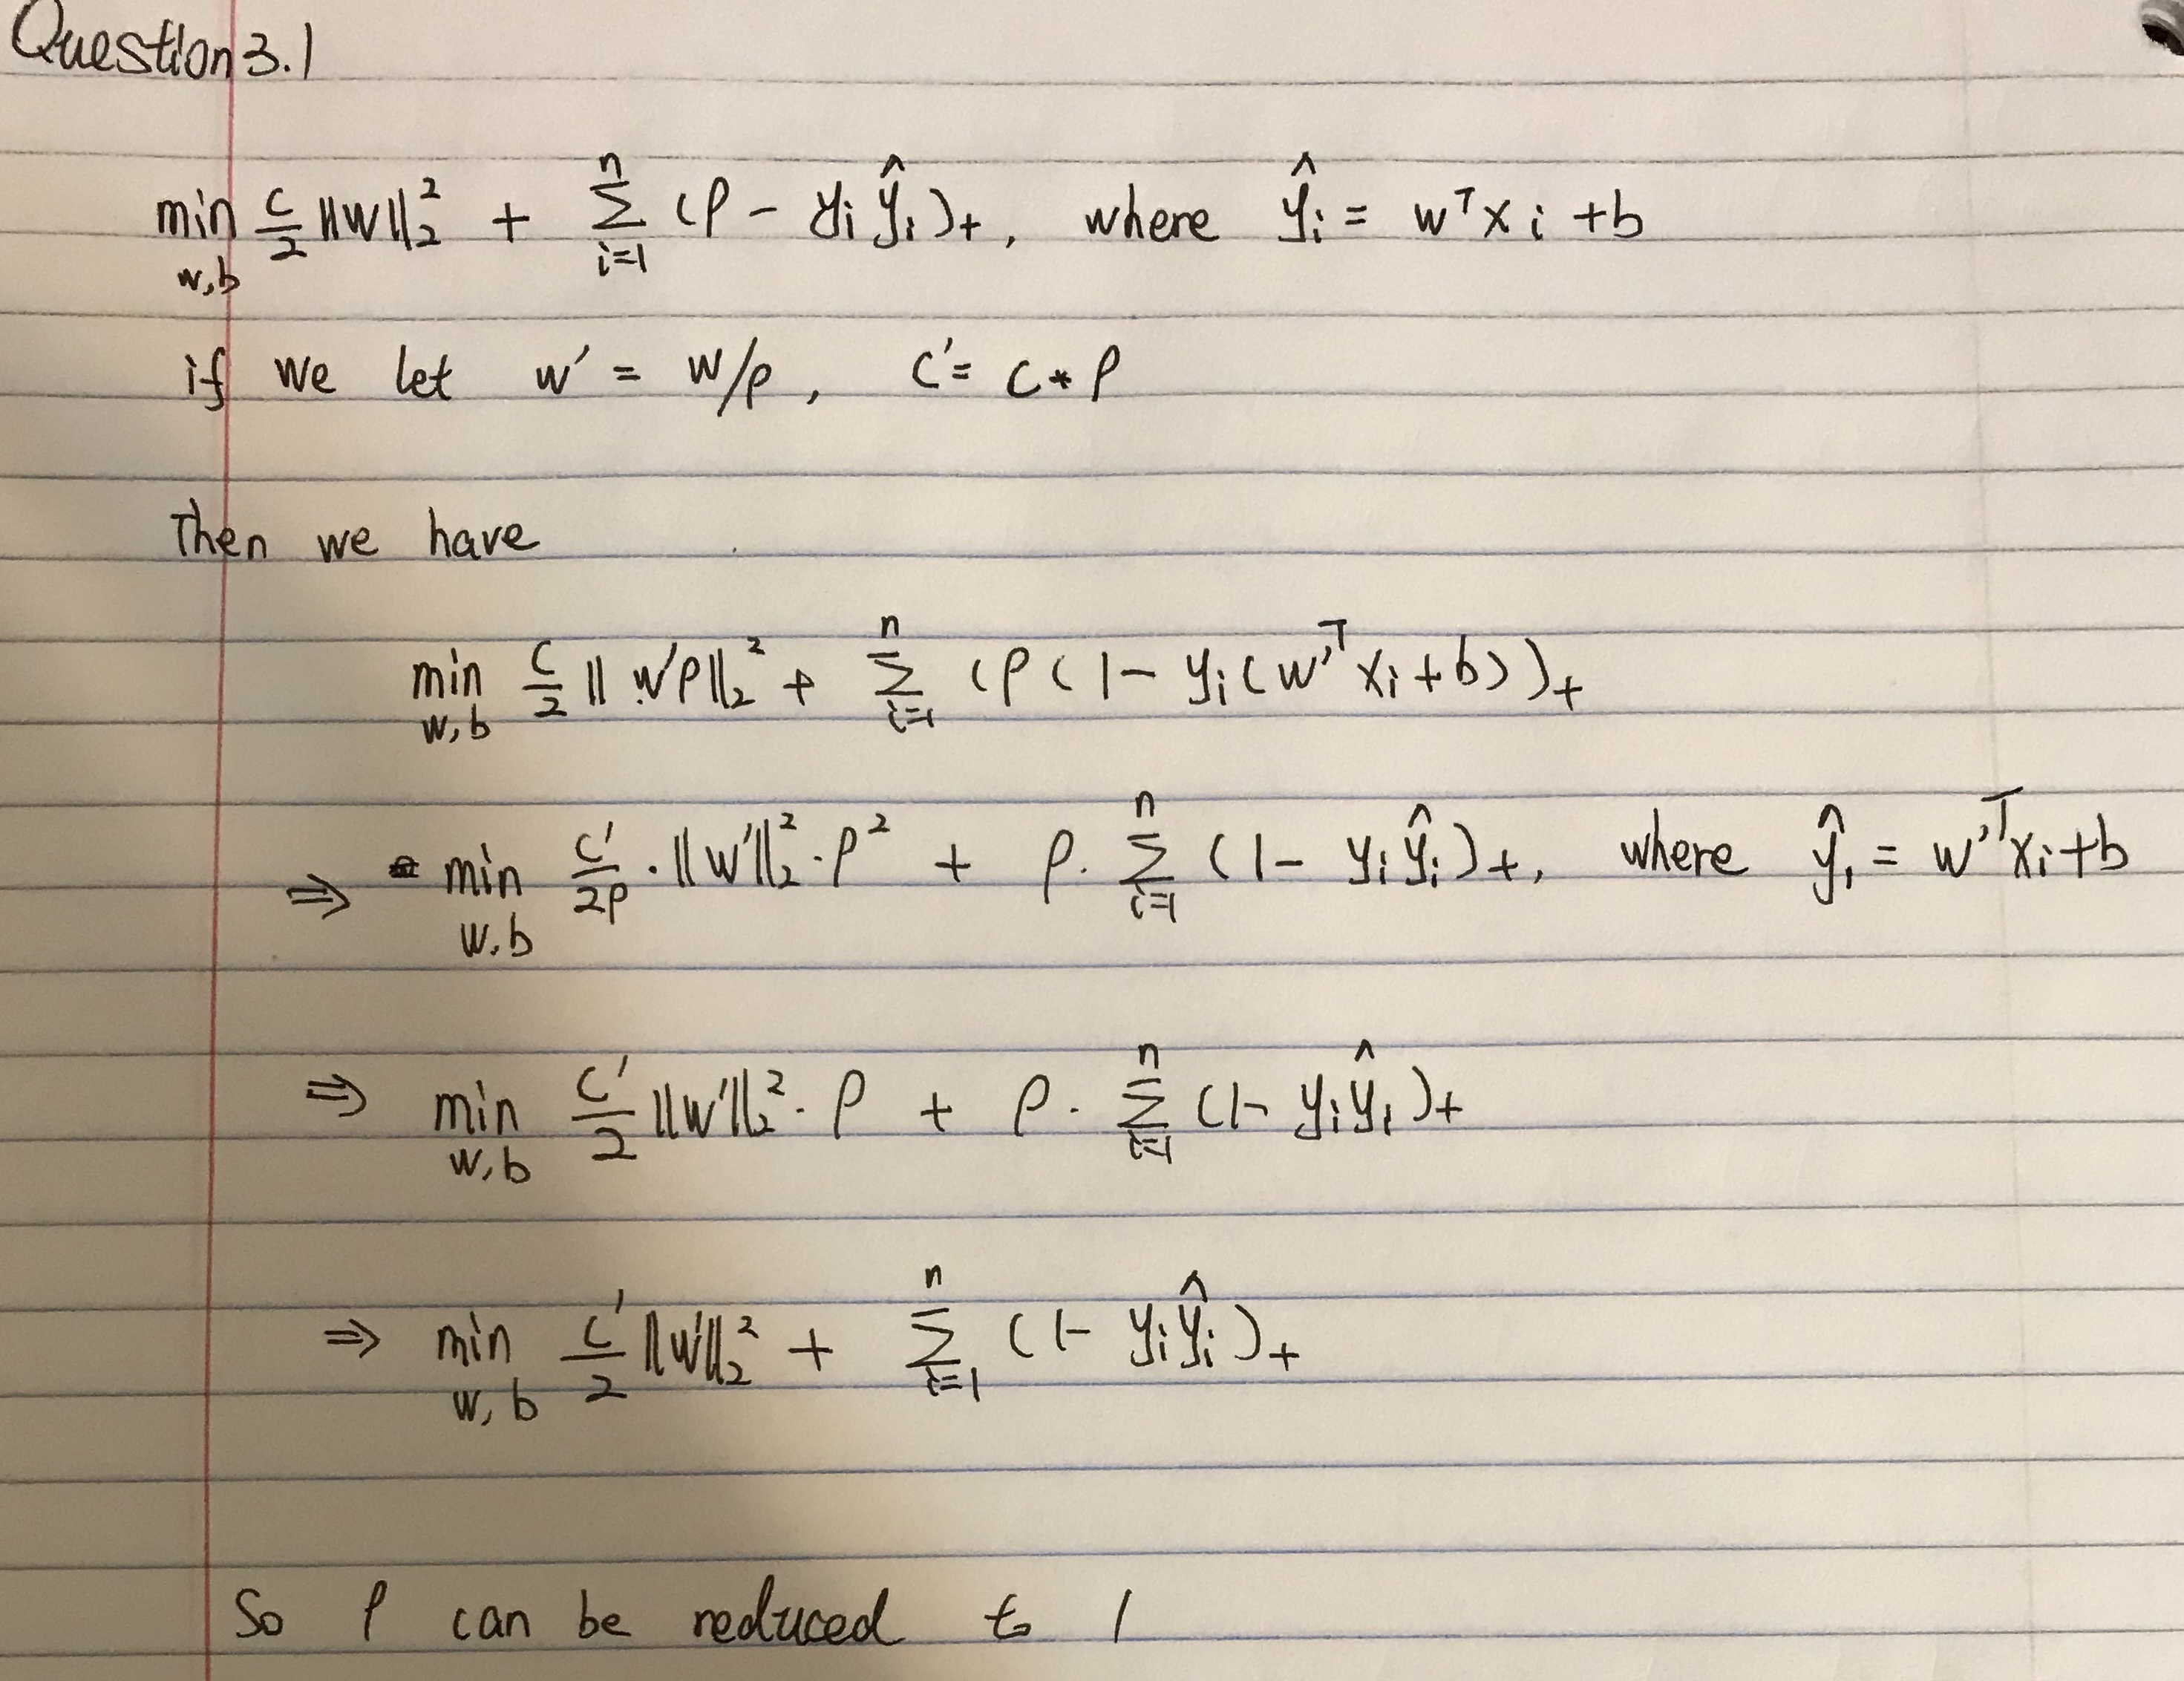
\includegraphics[scale=0.15]{q31.jpeg}]

\subsection{Question 3.2}
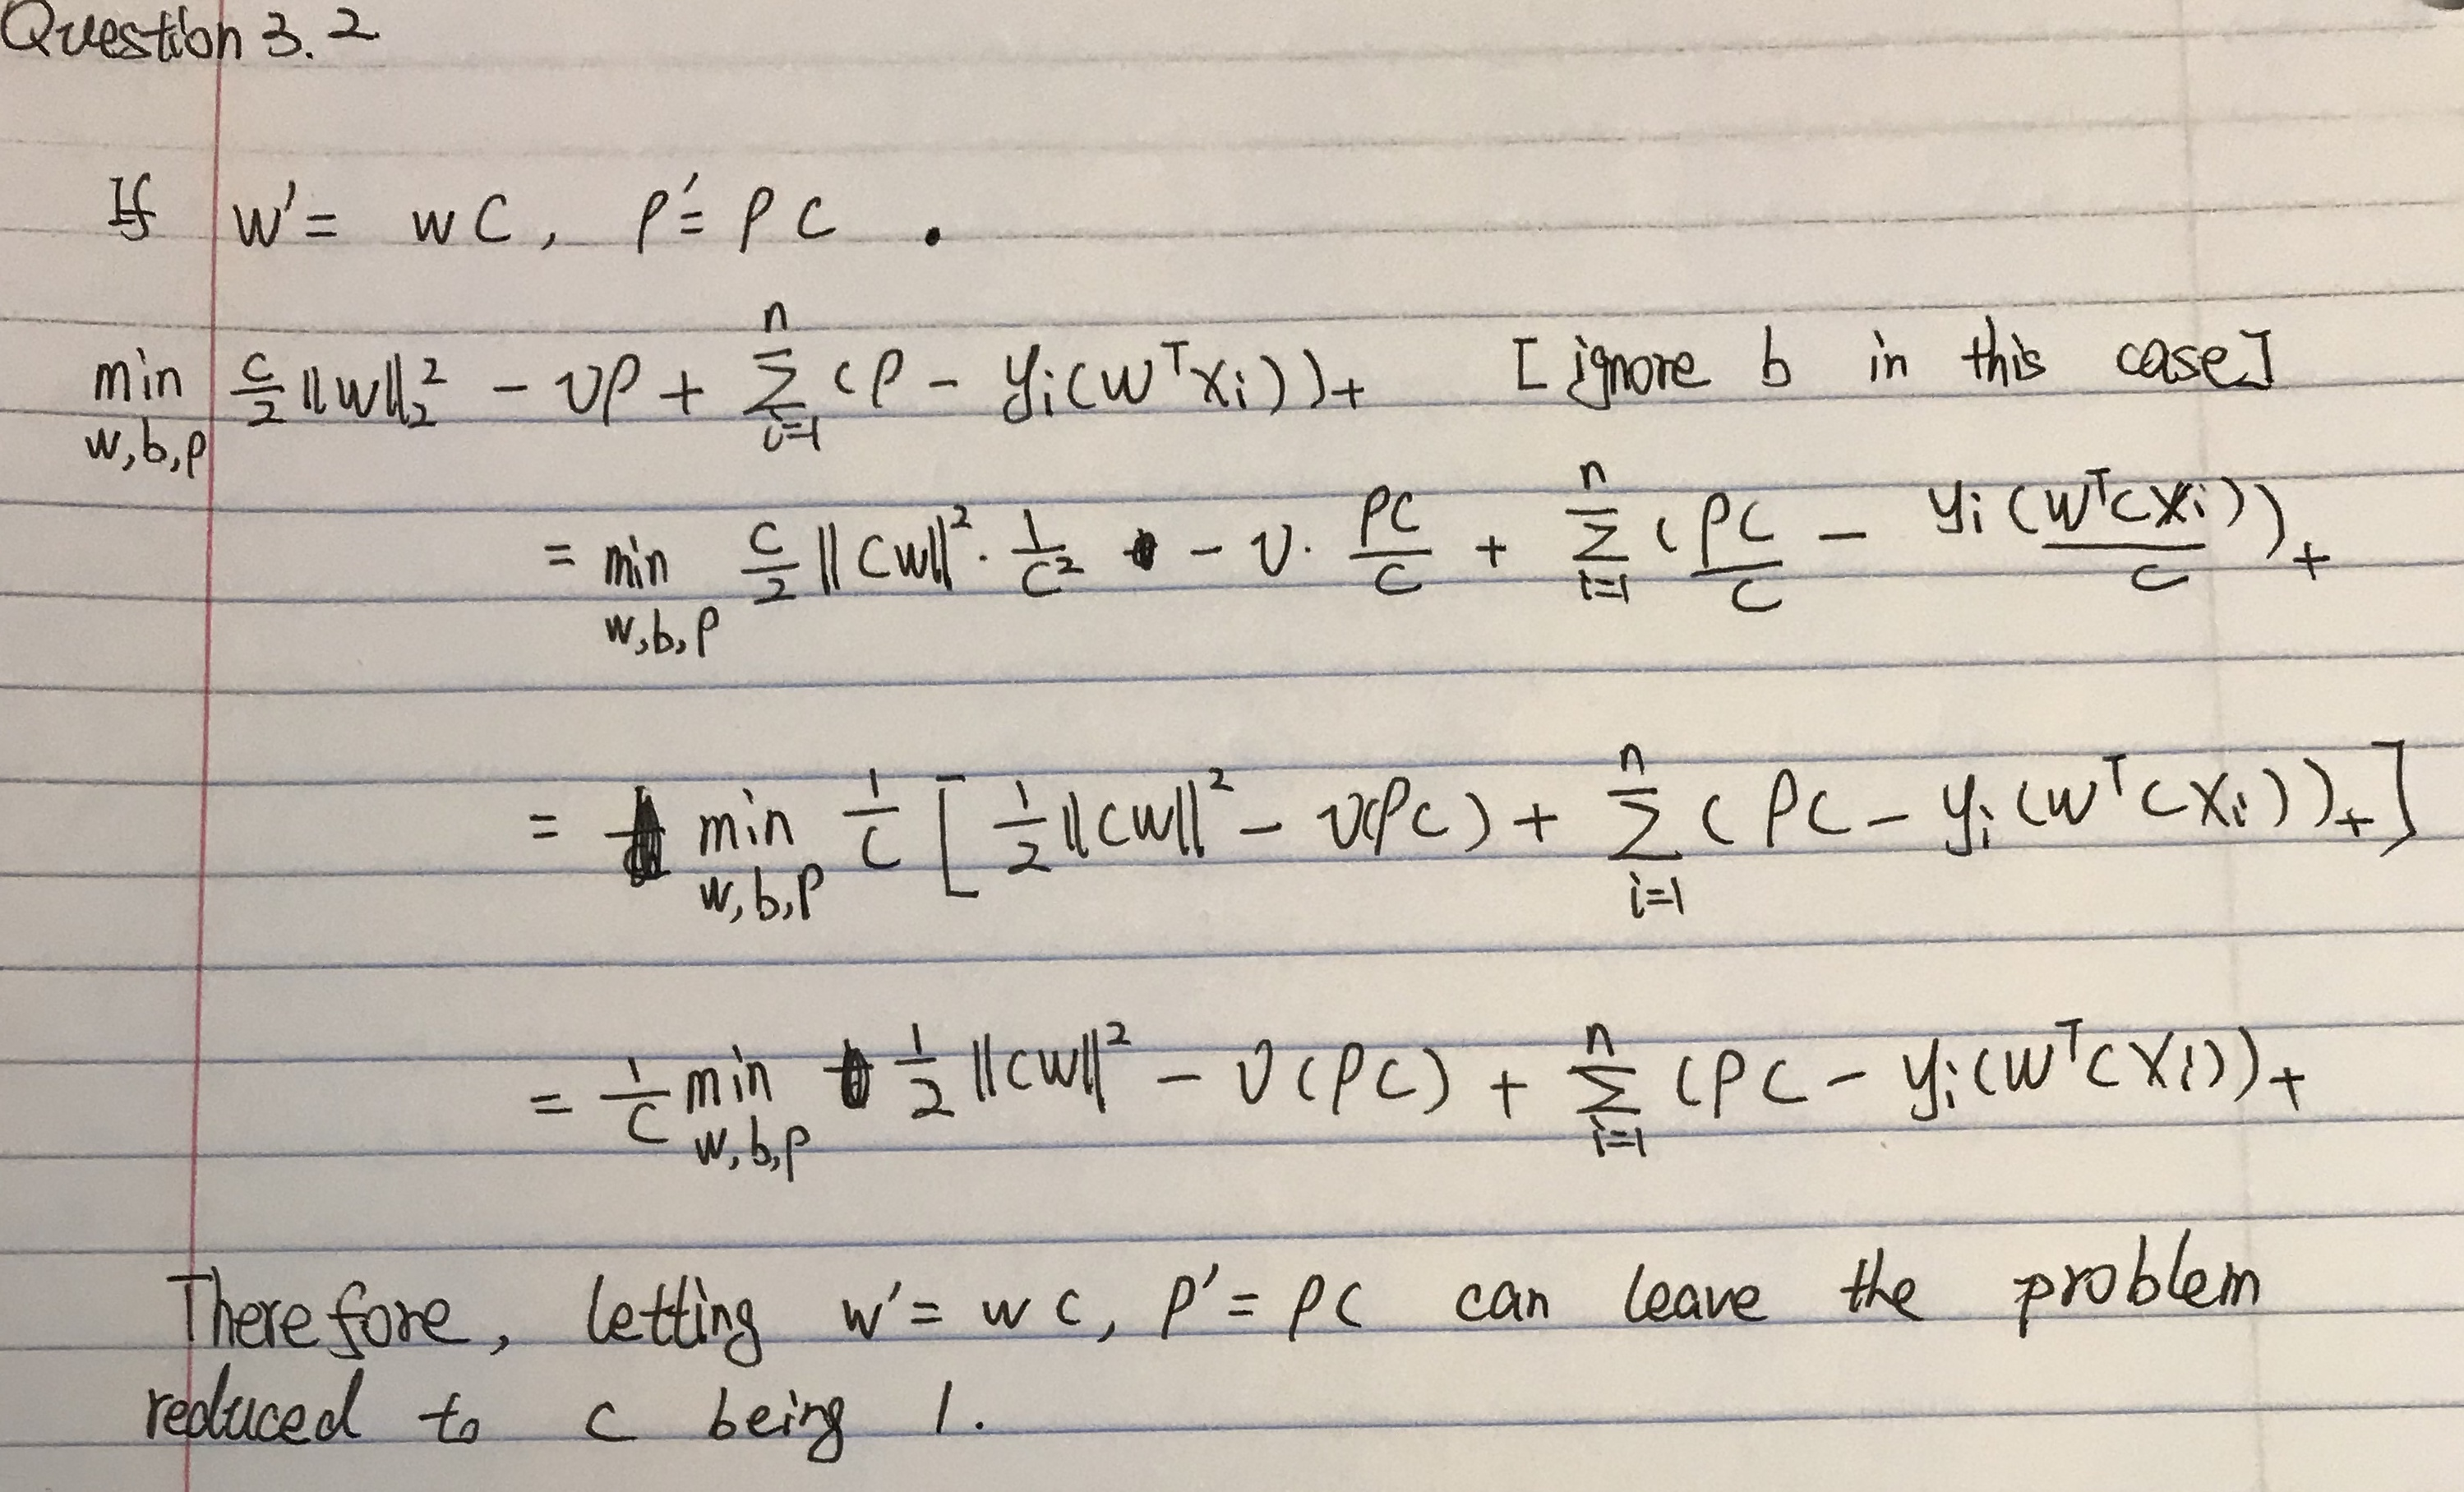
\includegraphics[scale=0.15]{q32.jpeg}]

\subsection{Question 3.3}
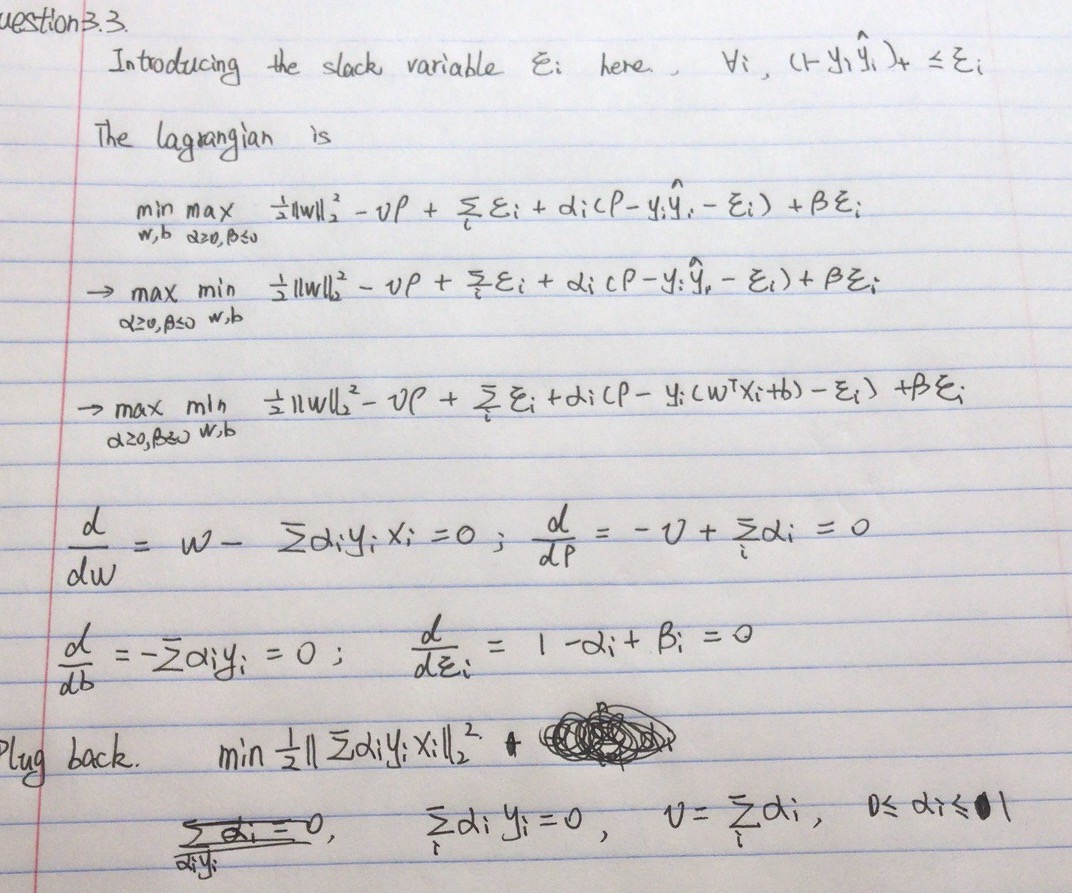
\includegraphics[scale=0.45]{q33.JPG}]

\subsection{Question 3.4}
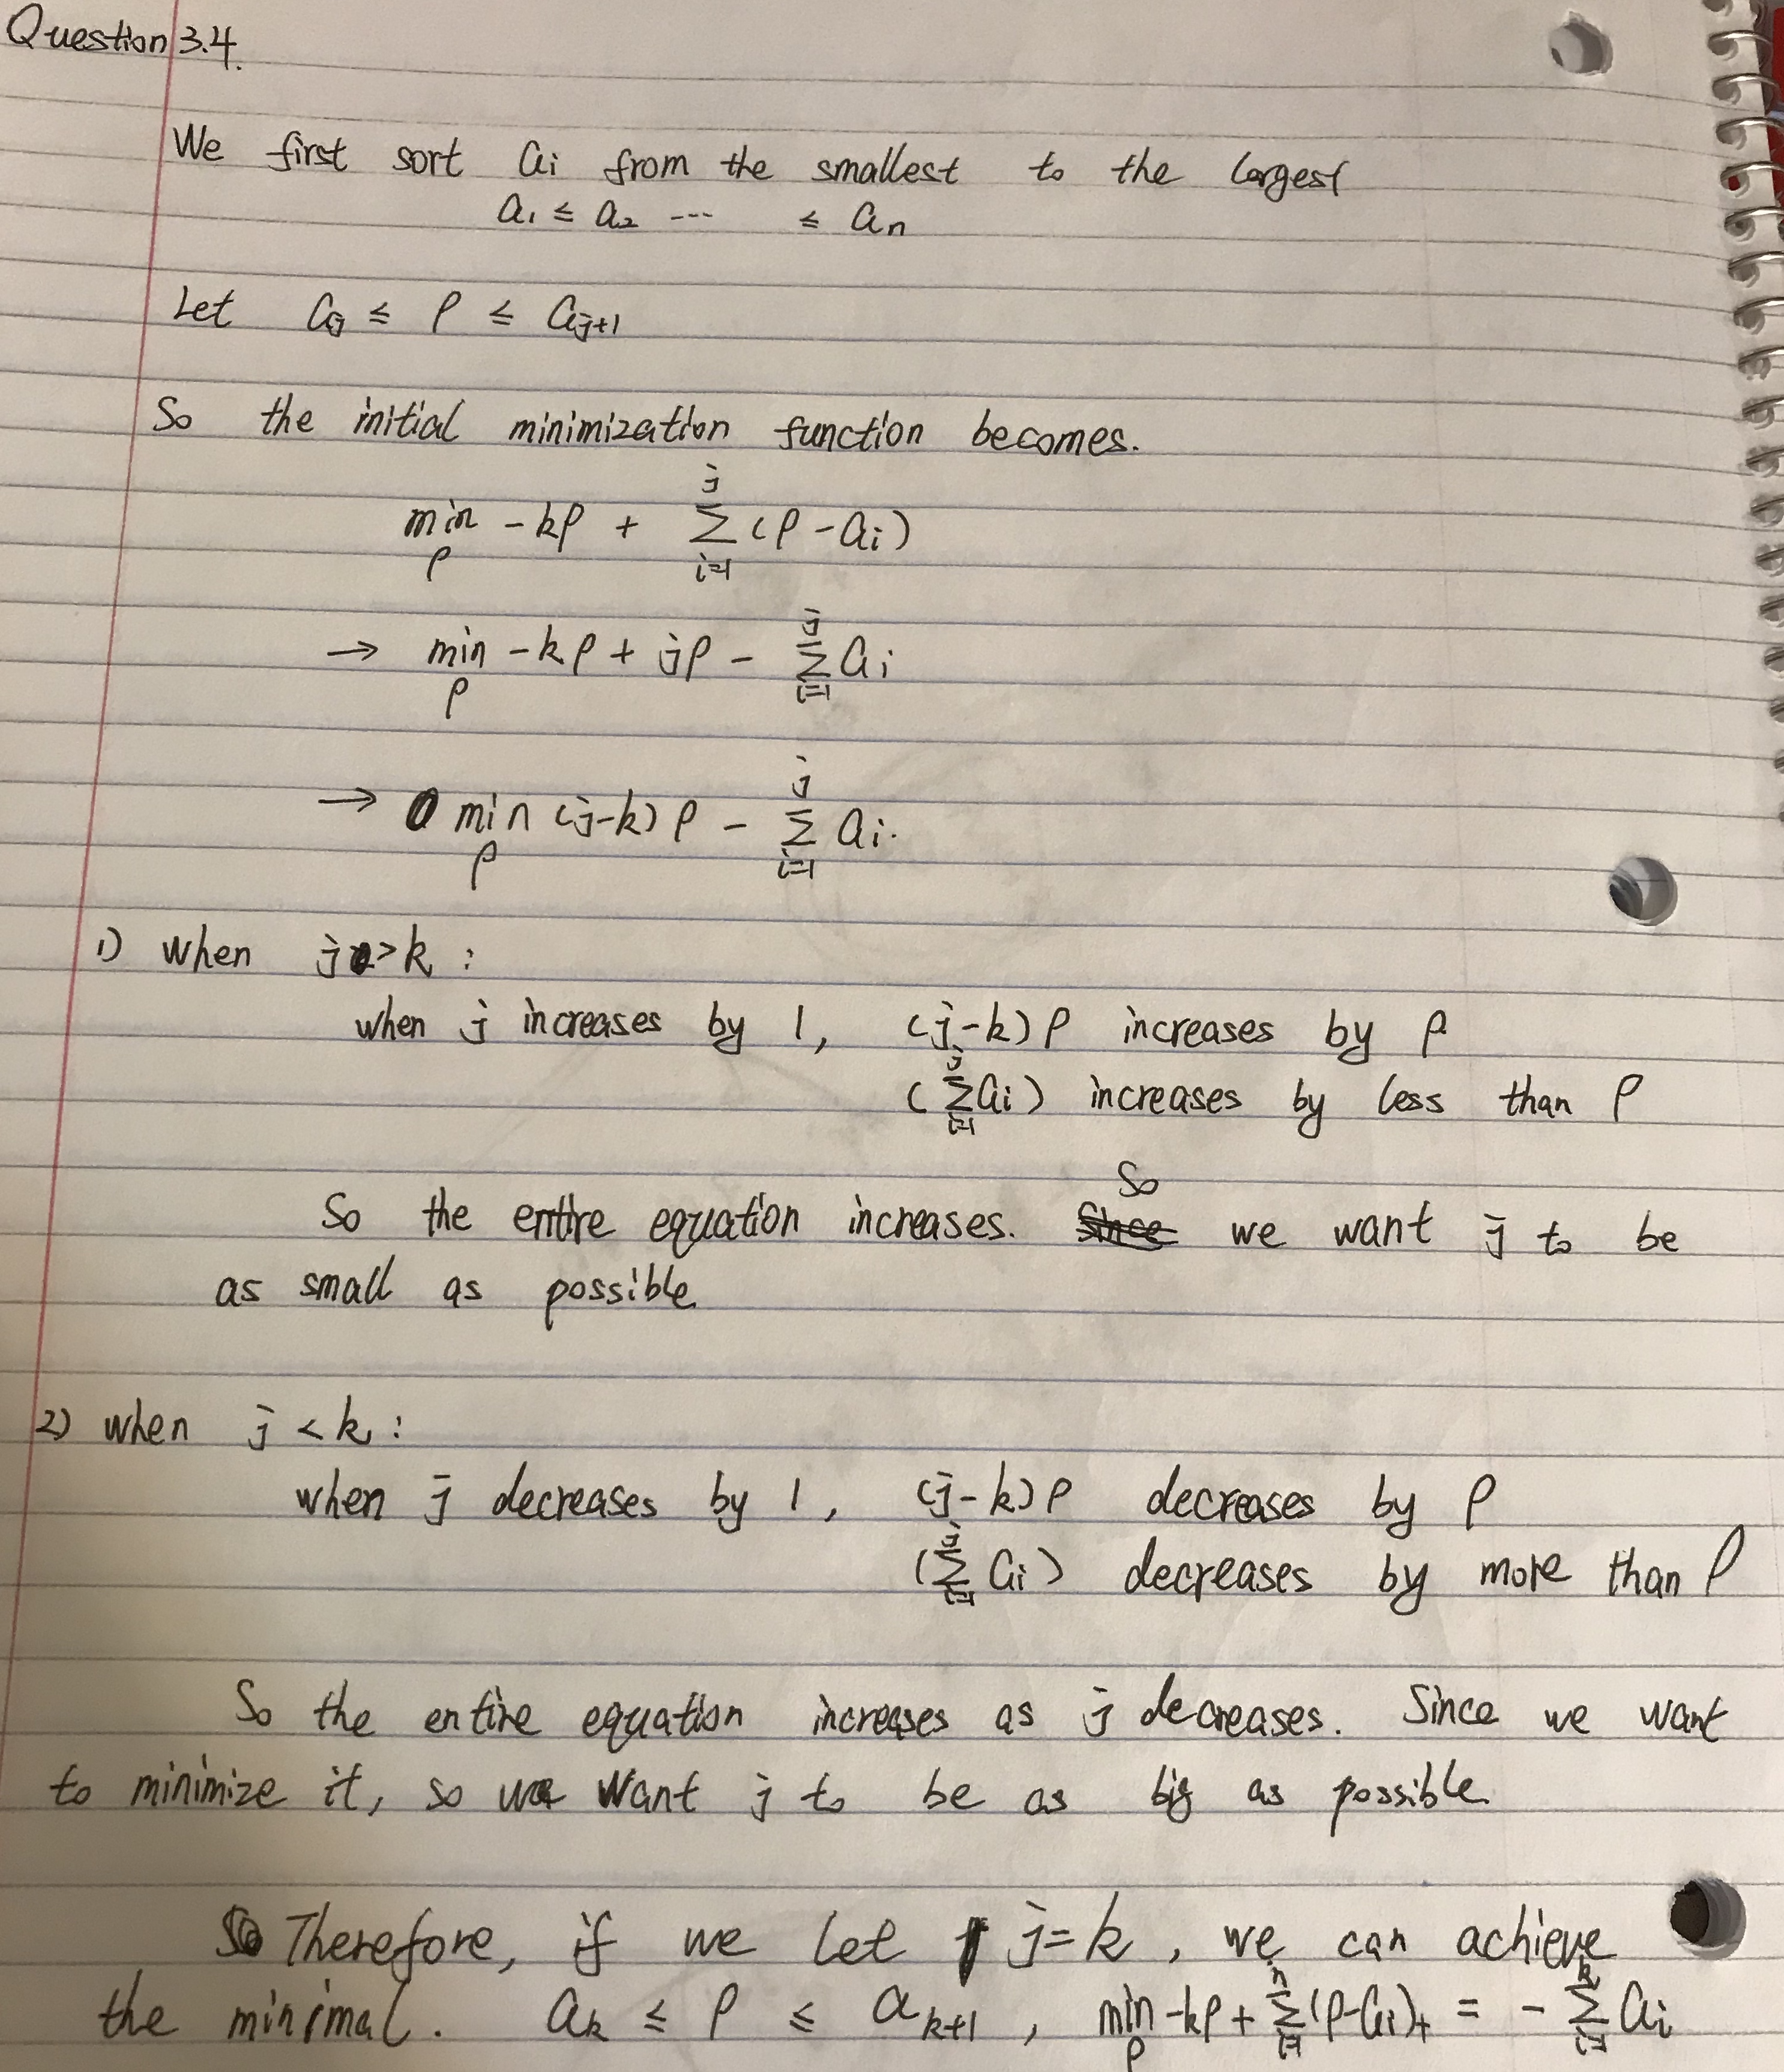
\includegraphics[scale=0.16]{q34.jpeg}]

\subsection{Question 3.5}
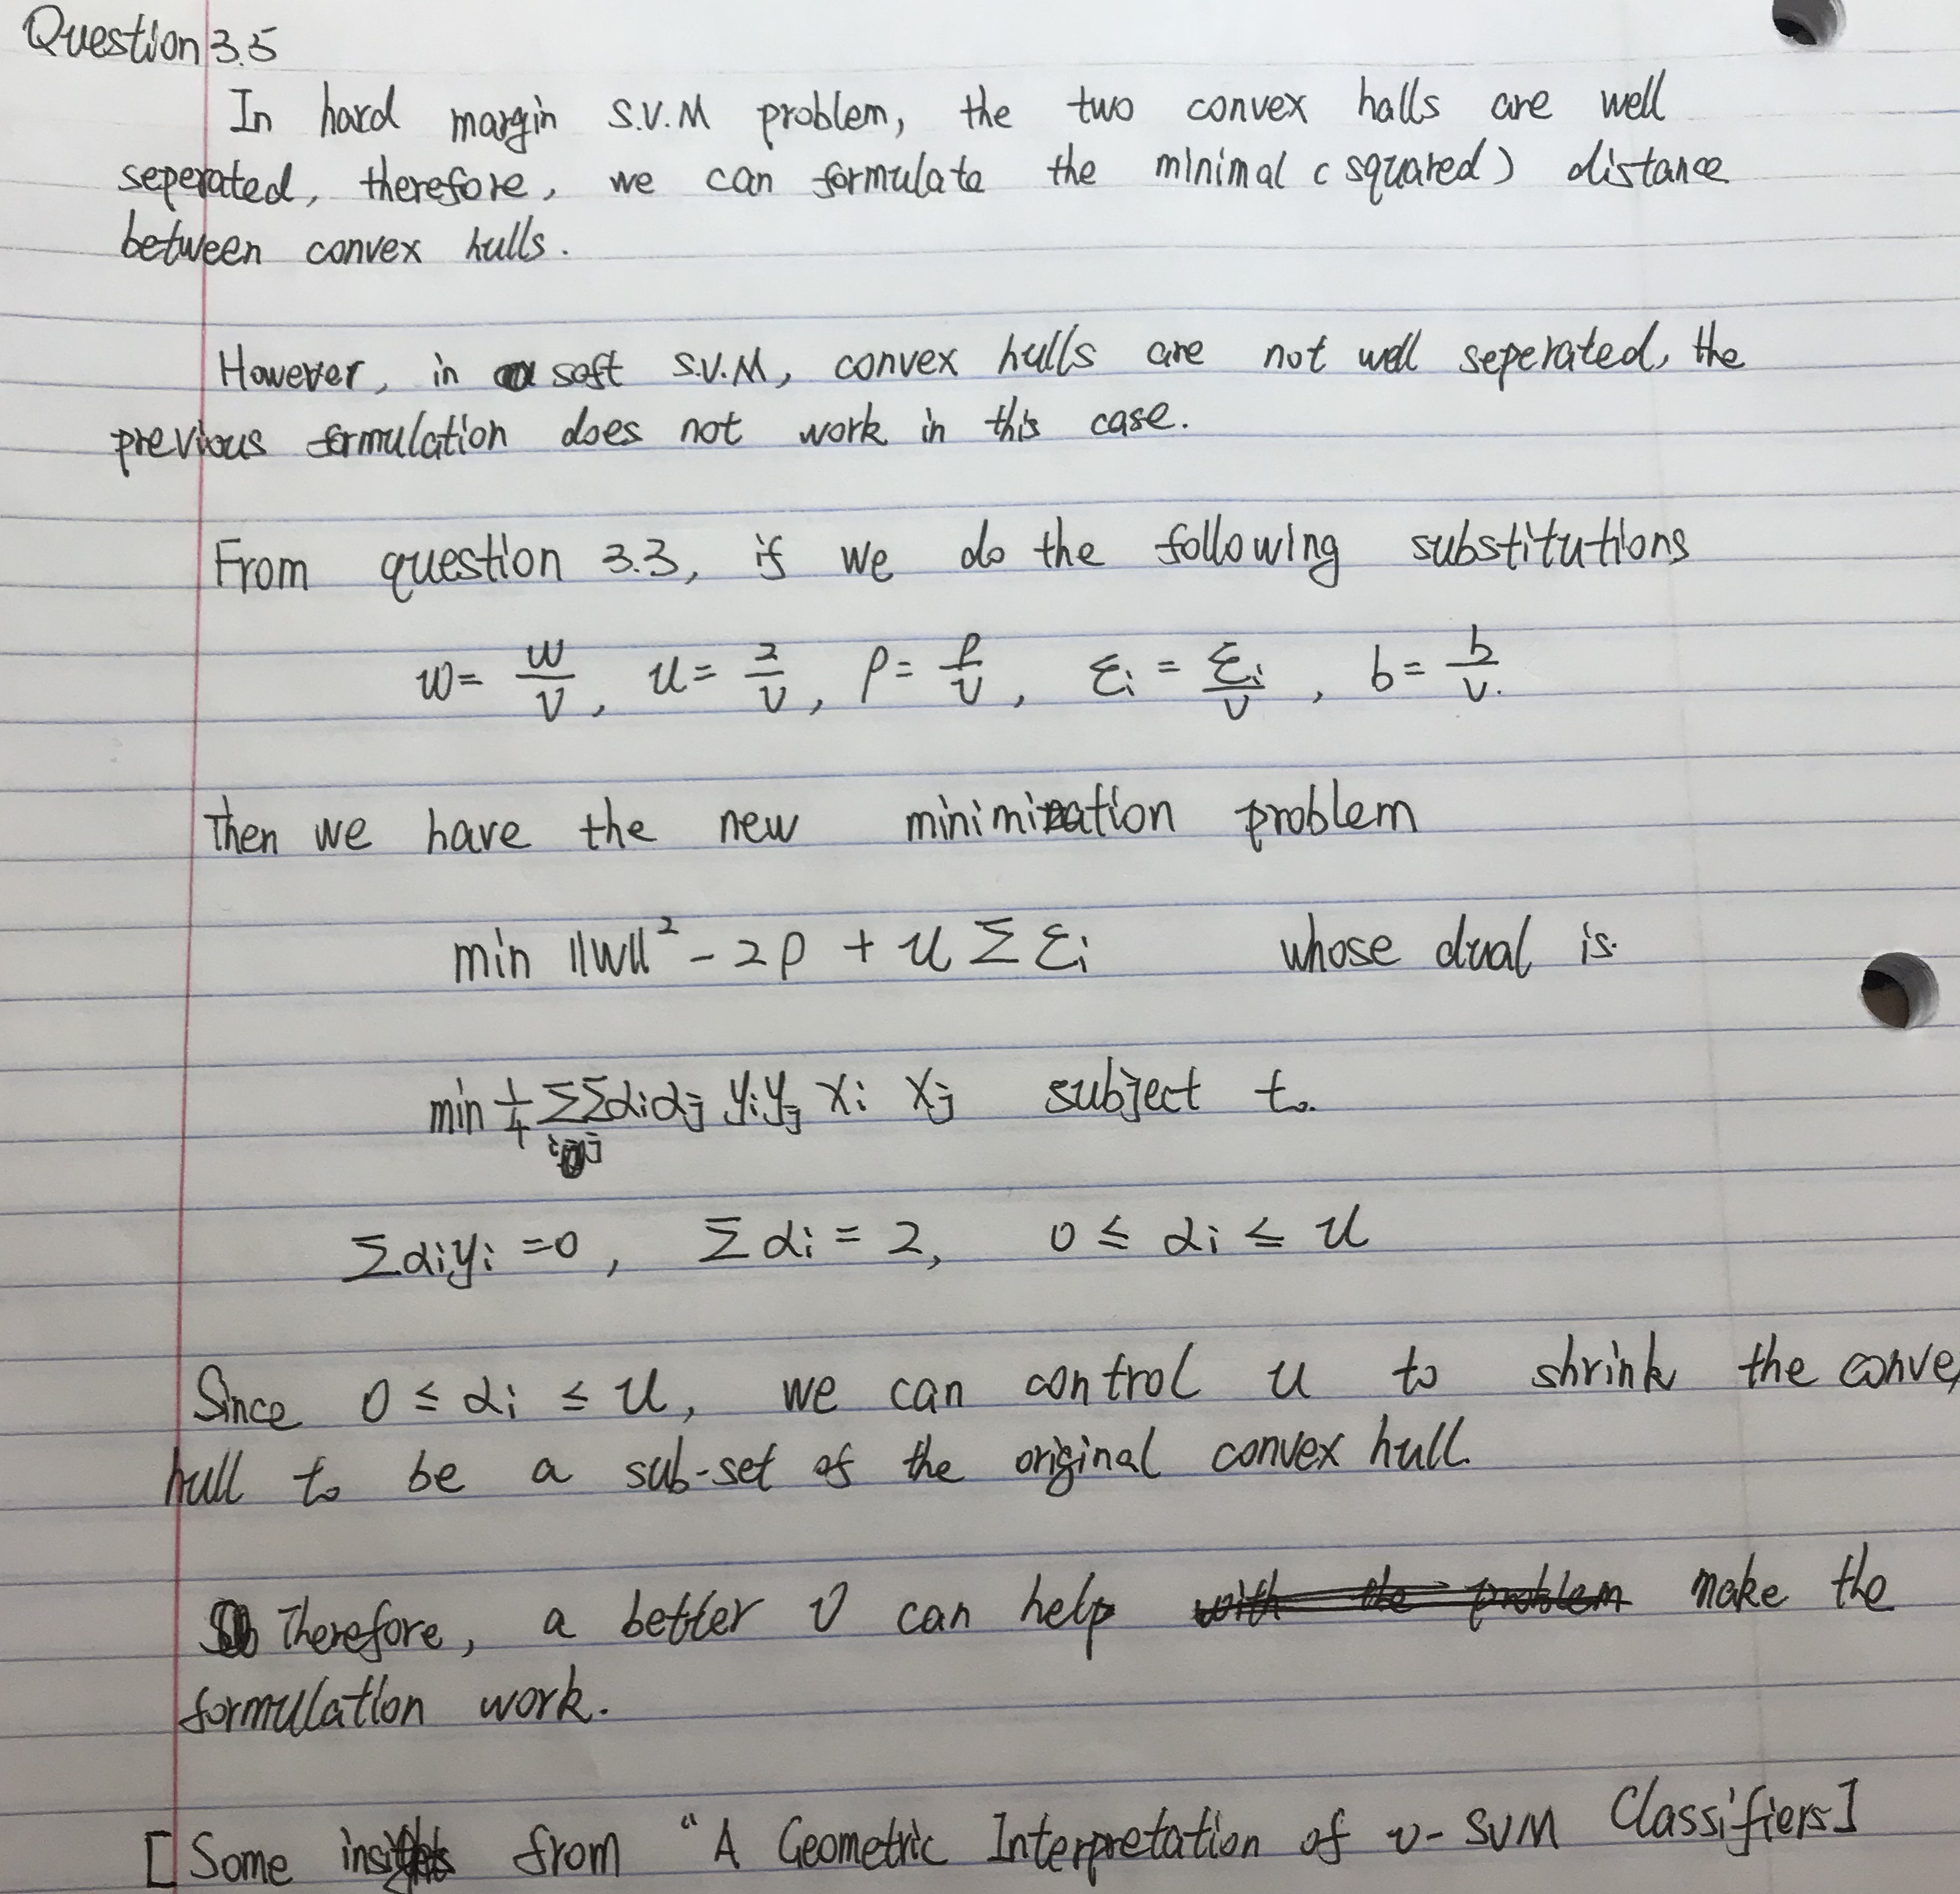
\includegraphics[scale=0.16]{q35.jpeg}]



\end{document}
